\documentclass{article}

\usepackage[utf8]{inputenc}
\usepackage{pgfplots}
\pgfplotsset{compat=1.18, width=10cm}

\begin{document}

\section{2D Plots}
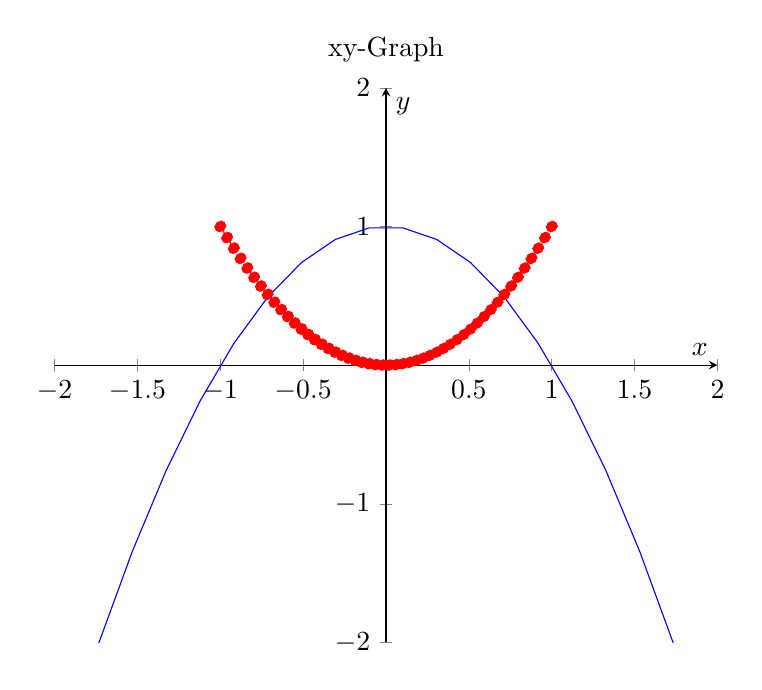
\begin{tikzpicture}
	\begin{axis}[xmin=-2, xmax=2, ymin=-2, ymax=2,
		axis lines=middle,
		xlabel=$x$, ylabel=$y$, title={xy-Graph}]
		\addplot[color=red, samples=50, dashed, mark=*, domain=-1:1]{x^2};
		\addplot[color=blue, samples=50]{1-x^2};
	\end{axis}
\end{tikzpicture}

\begin{tikzpicture}
	\begin{axis}[clip=false,
		xmin=0, xmax=2.5*pi, ymin=-1.5, ymax=1.5, axis lines=middle,
		xtick={0, pi/2, pi, 3*pi/2, 2*pi},
		xticklabels={$0$, $\frac{\pi}{2}$, $\pi$, $\frac{3 \pi}{2}$, $2 \pi$},
		xticklabel style={anchor=south west}, xmajorgrids = true, grid style=dashed]
		\addplot[domain=0:2*pi, red]{sin(deg(x))}
		node[right, pos=0.9]{$f(x)=\sin x$};
		\addplot[domain=0:2*pi, blue]{cos(deg(x))}
		node[right, pos=1]{$g(x)=\cos x$};
	\end{axis}
\end{tikzpicture}

\section{3D Plots}

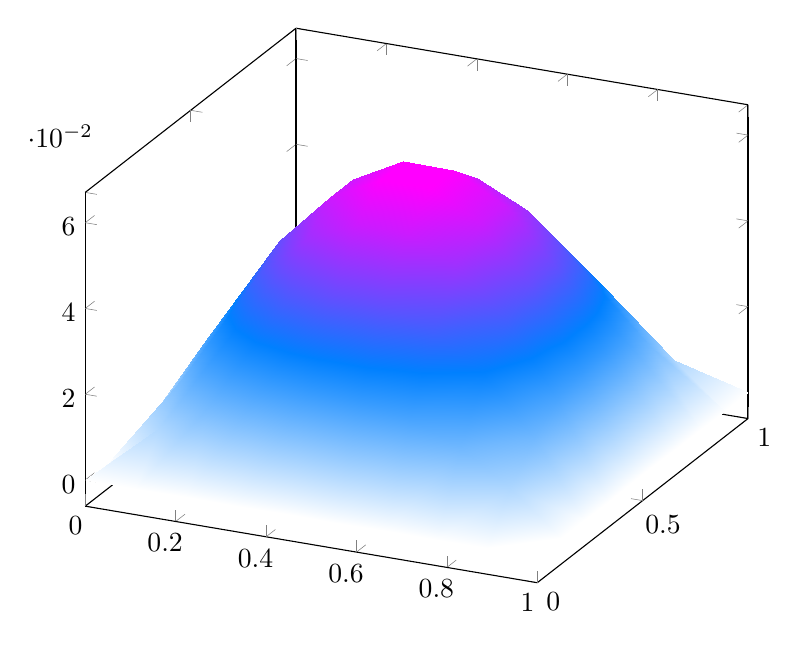
\begin{tikzpicture}
	\begin{axis}[colormap/cool]
		\addplot3[surf,samples=10,domain=0:1,
		shader=interp]
		{x*(1-x)*y*(1-y)};
	\end{axis}
\end{tikzpicture}

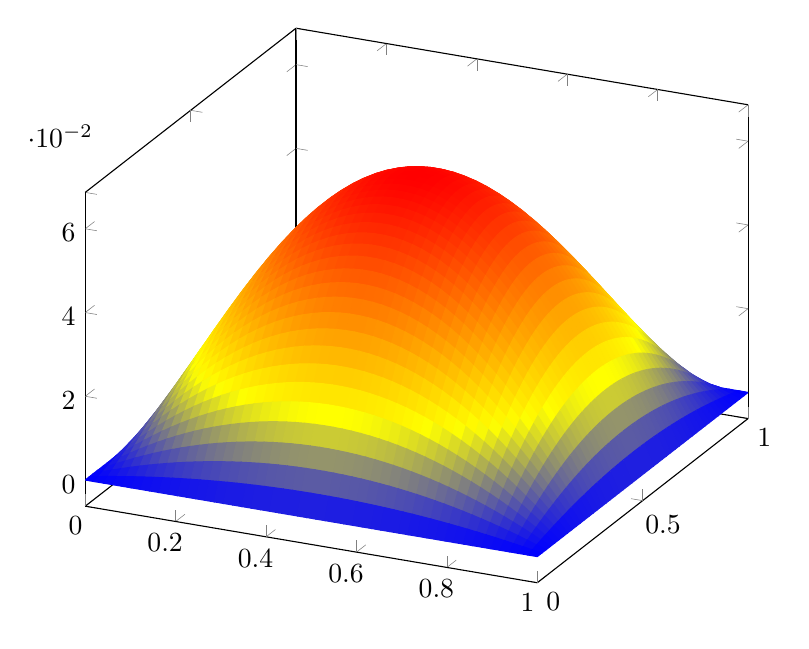
\begin{tikzpicture}
	\begin{axis}
		\addplot3[surf,samples=50,domain=0:1,
		shader=flat]
		{x*(1-x)*y*(1-y)};
	\end{axis}
\end{tikzpicture}

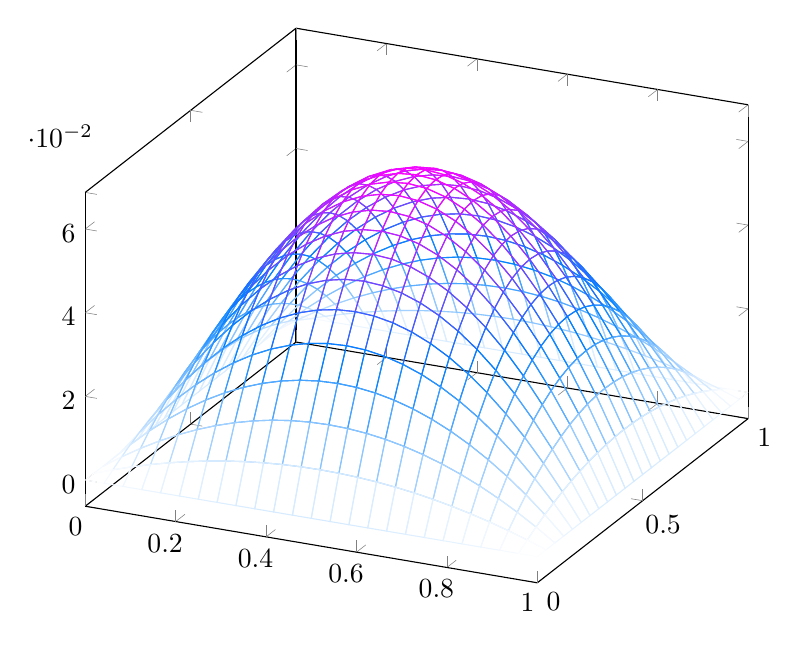
\begin{tikzpicture}
	\begin{axis}[colormap/cool]
		\addplot3[mesh,samples=25,domain=0:1,
		shader=flat]
		{x*(1-x)*y*(1-y)};
	\end{axis}
\end{tikzpicture}

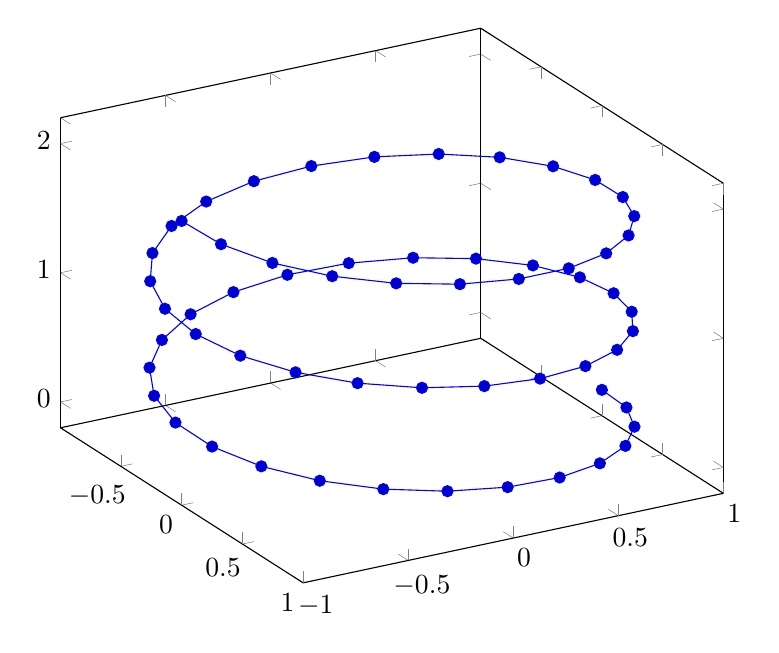
\begin{tikzpicture}
	\begin{axis}[view={60}{30}]
		\addplot3+[domain=0:5*pi,samples=60,samples y=0]
		({sin(deg(x))},
		{cos(deg(x))},
		{2*x/(5*pi)});
	\end{axis}
\end{tikzpicture}

\end{document}